\documentclass[paper=a4,fontsize=11pt]{scrartcl}
\usepackage[english]{babel}
\usepackage{graphicx}
\usepackage[svgnames]{xcolor}
\usepackage{geometry}
\textheight=650pt
\usepackage{url}
\usepackage{fontawesome5}
\usepackage[export]{adjustbox}
\usepackage{sectsty}
\usepackage{hyperref}
\usepackage{amsmath}

\frenchspacing
\pagestyle{empty}
\sectionfont
{
    \usefont{OT1}{phv}{b}{n}
    \sectionrule{0pt}{0pt}{-5pt}{3pt}
}

%%% Macros
%%% ------------------------------------------------------------
\newlength{\spacebox}
\settowidth{\spacebox}{8888888888}
\newcommand{\sepspace}{\vspace*{1em}}

\newcommand{\MyName}[1]{
        \Huge \usefont{OT1}{phv}{b}{n} \hfill #1
        \par \normalsize \normalfont}
		
\newcommand{\MySlogan}[1]{
		\large \usefont{OT1}{phv}{m}{n}\hfill #1
		\par \normalsize \normalfont}

\newcommand{\NewPart}[1]{\section*{\uppercase{#1}}}

\newcommand{\PersonalEntry}[2]{
		\noindent\hangindent=0em\hangafter=0
		\parbox{\spacebox}{#1}
		\hspace{2.5em} #2 \par}

\newcommand{\SkillsEntry}[4]{
		\noindent \textbf{#1} \hfill
		\colorbox{White}{\color{White}#2} \par
		\noindent #3 \par
		\noindent\hangindent=2em\hangafter=0 \small #4
		\normalsize \par}

\newcommand{\EducationEntry}[4]{
		\noindent \textbf{#1} \hfill
		\colorbox{Black}{
			\parbox{6em}{
			\hfill\color{White}#2}} \par
		\noindent #3 \par
		\noindent\hangindent=2em\hangafter=0 \small #4
		\normalsize \par}

\newcommand{\WorkEntry}[4]{
		\noindent \textbf{#1} \hfill
		\colorbox{Black}{\color{White}#2} \par
		\noindent #3 \par
		\noindent\hangindent=2em\hangafter=0 \small #4
		\normalsize \par}

%%% ------------------------------------------------------------
\begin{document}

\noindent
\begin{minipage}[t]{3.8cm}
    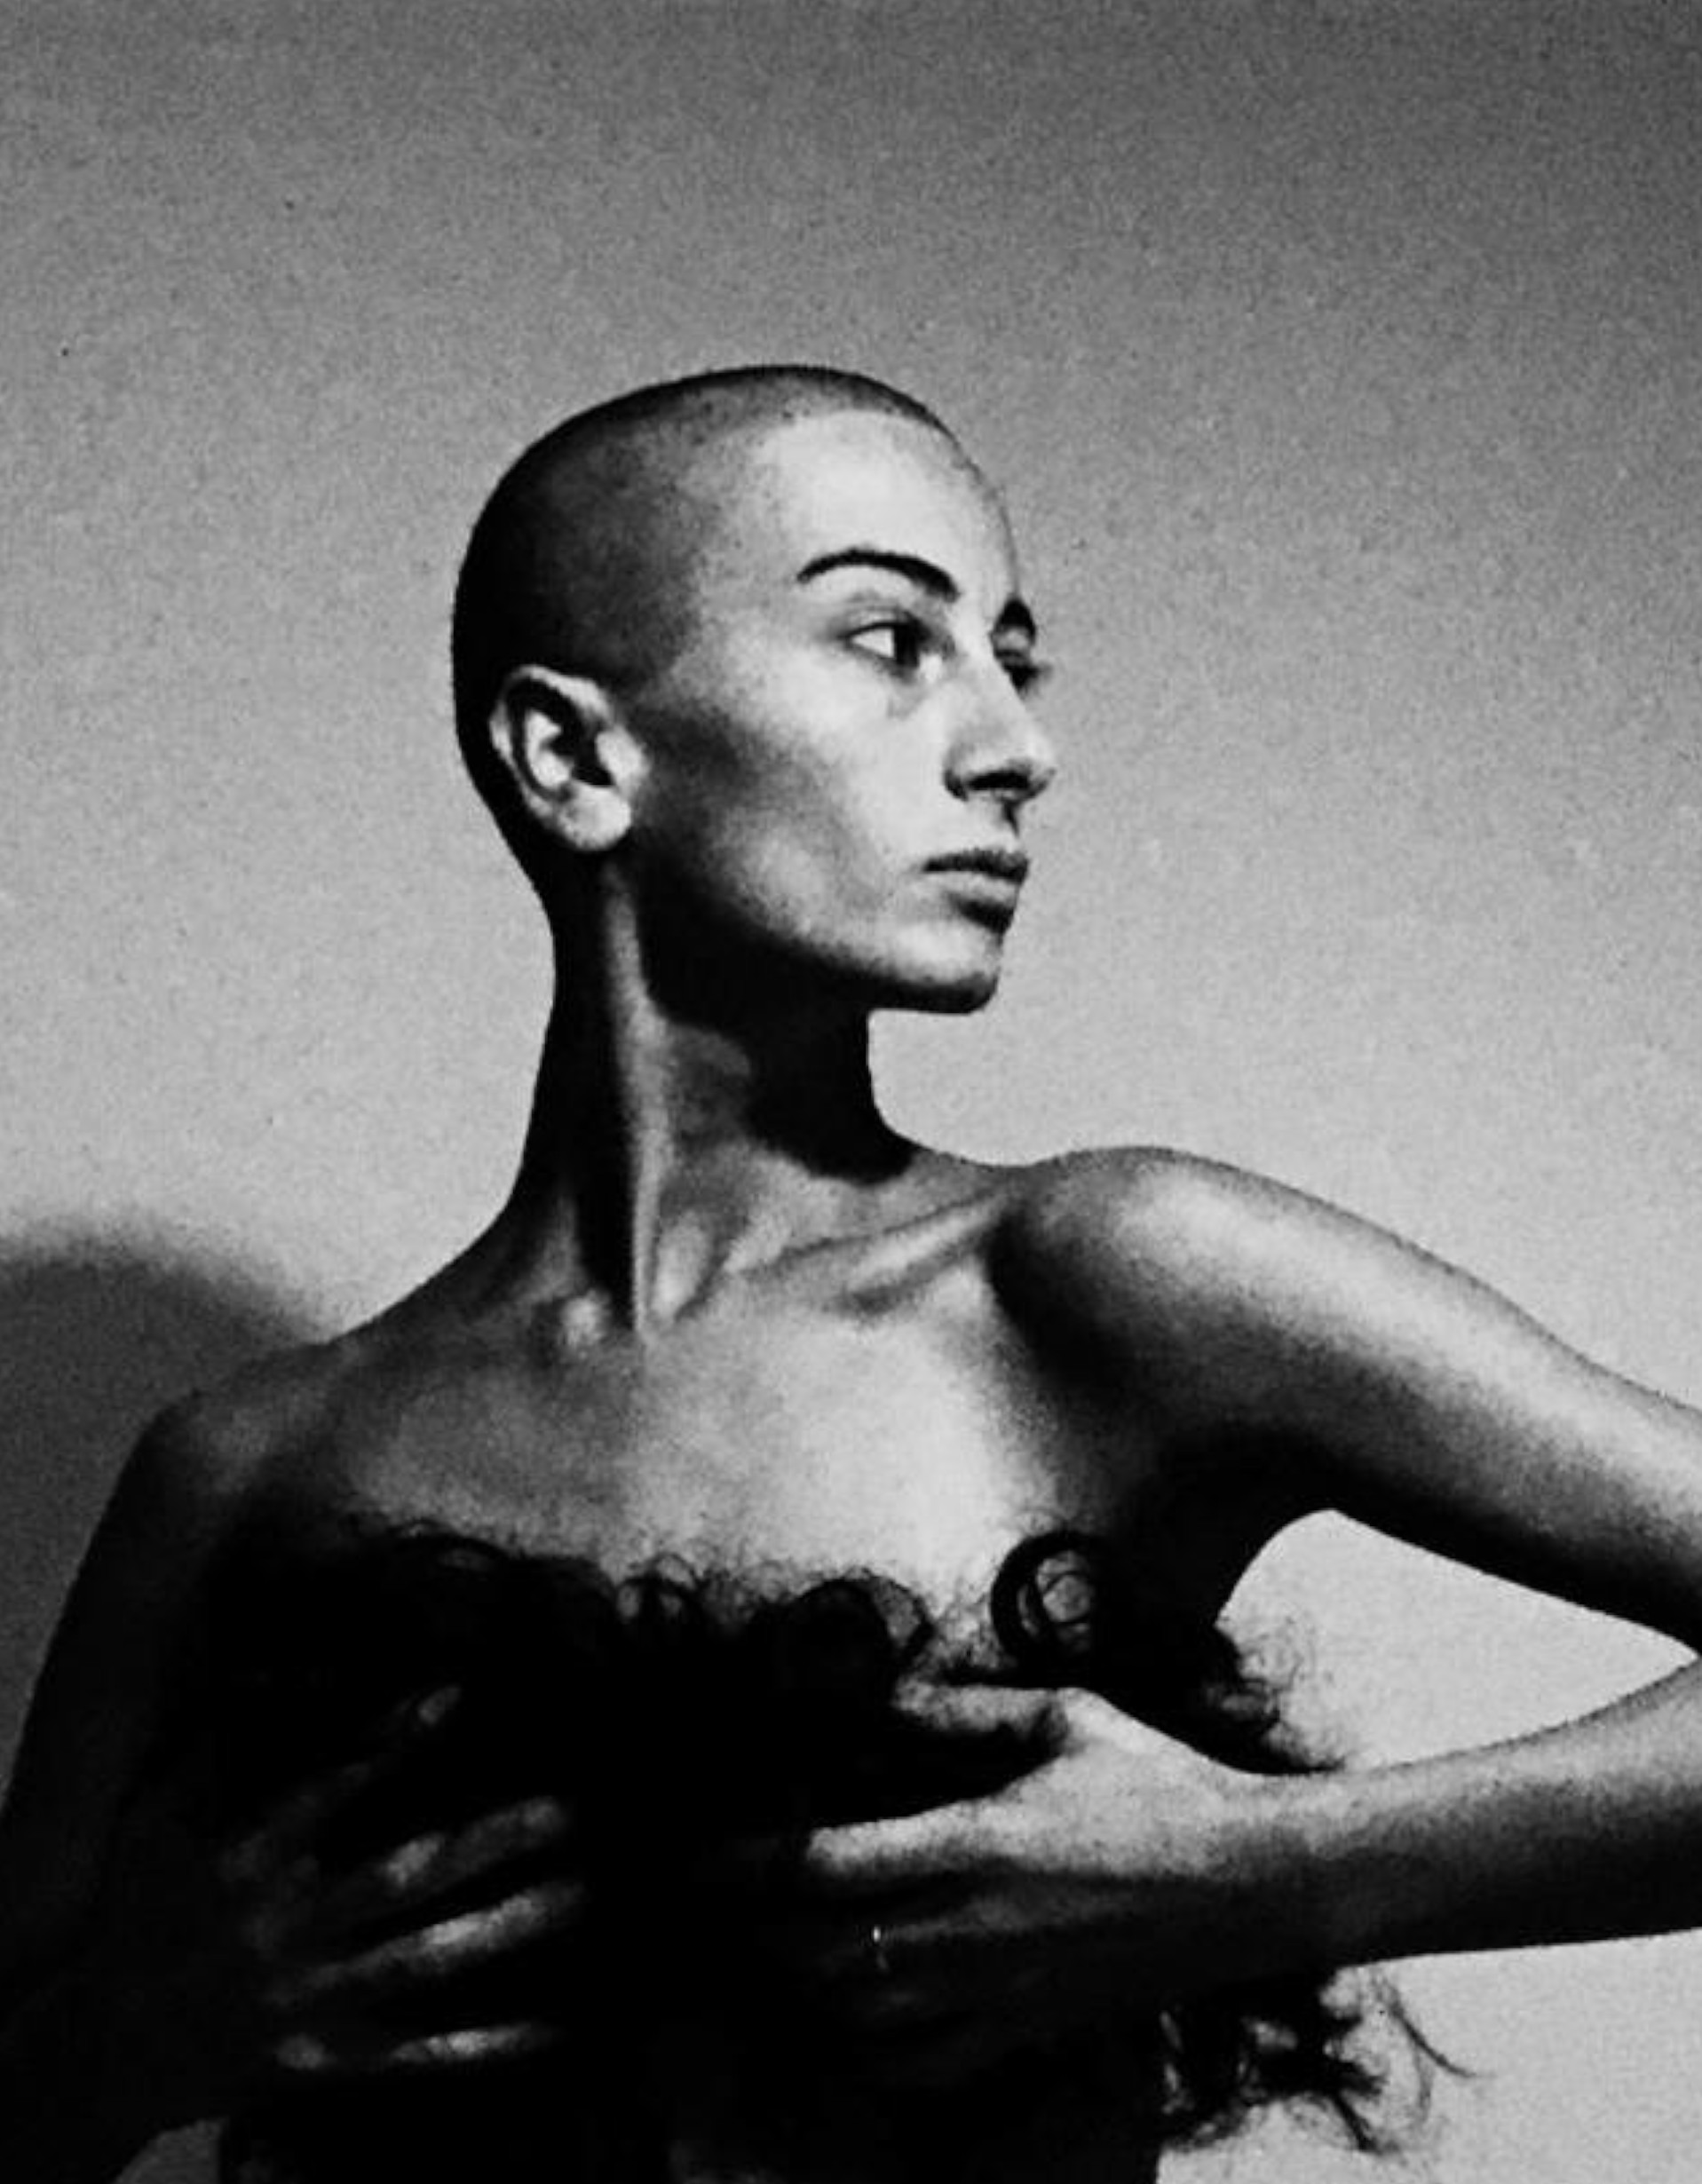
\includegraphics[height=4cm, valign=t]{images/portrait}
\end{minipage}
\hspace{1em}
\begin{minipage}[t]{0.7\textwidth}
    \MyName{Simon Zimmermann}
    \MySlogan{Software Developer}
    \sepspace
    \sepspace
    \sepspace

    \PersonalEntry{Birth}{June 5, 1993}
    \PersonalEntry{Location}{Düsseldorf, Germany}
    \PersonalEntry{Mail}{\url{mail@simonzimmermann.com}}
    \PersonalEntry{Github}{\faGithub\space\url{github.com/SimonZimmer}}
\end{minipage}

%%% ------------------------------------------------------------
\NewPart{Work Experience}{}
\EducationEntry{C++ Backend Software Developer}{2022-present}{Dear Reality GmbH, Full-time}{Backend research and development of DSP-algorithms and API design using C, C++ and Python}
\sepspace
\EducationEntry{C++ Fullstack Software Developer}{2020-present}{Dear Reality GmbH, Full-time}{Full-stack development of real-time audio applications following test-driven development, modern C++ and agile project management principles}
\sepspace
\EducationEntry{Researcher/QA Engineer (Working Student)}{2017-2020}{Dear Reality GmbH, Part-time}{Research and development of DSP prototypes, quality assurance, and test automation development}
\sepspace
\EducationEntry{Room-Acoustics Engineer (Working Student)}{2016-2017}{ISRW-Klapdor, Part-time}{Simulation of room-acoustic properties and in-situ acoustic measurements}

%%% ------------------------------------------------------------
\NewPart{Projects}{}
\EducationEntry{dearVR Exoverb}{2022}{Backend Developer}{Developed the DAW-plugin "Exoverb," which uses synthesized reverb impulse responses and additional processing to generate realistic reverberation effects}
\sepspace
\EducationEntry{Team Split Facilitation}{2022}{Backend Developer, DevOps Engineer}{Facilitated the transition from a single-team solution to a frontend/backend split. Extended the technology stack with Conan, Microsoft Azure, Pure Data, and C}
\sepspace
\EducationEntry{dearVR MIX/MONITOR}{2021}{Full Stack Developer}{Developed the multichannel DAW-plugins "dearVR MIX" and "dearVR MONITOR," which utilize headphone calibration, room simulation and binauralization to virtualize studio environments}

\NewPart{Publication}{}
\EducationEntry{Co-Author}{2021}{Conference Paper}{Immersive and 3D Audio: from Architecture to Automotive (I3DA): "Machine Learning-Based Room Classification for Selecting Binaural Room Impulse Responses in Augmented Reality Applications"}

%%% ------------------------------------------------------------
\NewPart{Education}{}
\EducationEntry{M.Sc. Media Informatics}{2018-2020}{University of Applied Sciences Düsseldorf}{Thesis title: 'Scalable Modelling of Room Acoustic Characteristics for AR-devices on the Basis of Visual Information Using Deep Learning' - honors degree}
\sepspace
\EducationEntry{M.Sc. Music Informatics}{2018}{University of Music Karlsruhe}{Guest Semester}
\sepspace
\EducationEntry{B.Eng. Media Engineering}{2012-2017}{University of Applied Sciences Düsseldorf}{Thesis title: 'A Concept for Implementing Room Acoustic Properties in the Context of a 3D-Audio Engine'}

%%% ------------------------------------------------------------
\NewPart{Skills}{}
\SkillsEntry{Languages}{}{}{German (native), English (fluent)}
\sepspace
\SkillsEntry{Technologies}{}{}{\textsc{C++17}, C99, boost, CMake, conan, Python, googletest/googlemock, google benchmark, Pure Data (Pd), Azure DevOps, Github Actions, Jenkins, git, docker, JUCE, pybind11, flask, wagtail, MATLAB, \LaTeX, Linux, nvim/vim}
\sepspace
\SkillsEntry{Other}{}{}{Music Production, Modular Synthesizer, Esoteric Programming Languages (Orca, TidalCycles)}

\end{document}
